\section{OS API}

\subsection{Sub topics}

\begin{itemize}
	\item The design philosophy - Why OO and OS Api?
	\item Elaborate on the challenge of building it and its currenct design:
	\begin{itemize}
		\item The PIMPL / Cheshire Cat idiom - The how and why.
		\item CPU / OS Architecture.
	\end{itemize}
	\item Effect on design/implementation:
	\begin{itemize}
		\item MQs (Message queues) used with pthreads contra MQ used in OO OS Api.
		\item RAII in use.
		\item Using Threads before and now.
	\end{itemize}
	\item UML Diagrams to implementation (class and sequence) - How?
\end{itemize}

\subsection{Curriculum}

\begin{itemize}
	\item Slides: OS Api".
	\item OLA: OSAL SERNA SAC10".
	\item OLA: Speciffcation of an OS Api".
	\item Kerrisk: Chapter 35: Process Priorities and Schedul-ing".
\end{itemize}

\subsection{Exercises}

\begin{itemize}
	\item OS API.
\end{itemize}

\subsection{The design philosophy - Why OO and OS Api?}

Et OS Api giver et abstraktionslag for operativsystemet. Denne abstraktion gør det muligt at \textit{unify} OS arkitektur, og dermed opnå højere portabilitet for applikationer. \todo{ikke 'med' efter punktum}med andre ord giver et OS Api os et generelt interface der kan genbruges på tværs af platforme.

I vores tilfælde, i arbejdet med POSIX tråde, betyder et OS Api, at vi ikke skal omskrive vores kode, så den kan kompileres til Windows. Se illustration på figur \ref{fig:ApiModel}.
OS Api'et sikrer samtidigt at man ikke skal tænke på de lavpraktiske OS-spicifikke\todo{another goof} detaljer, og at man i stedet kan fokusere på brugbarheden af applikationen.

\todo{unfuck whitespace in fig}
\begin{figure}[h]
	\centering
	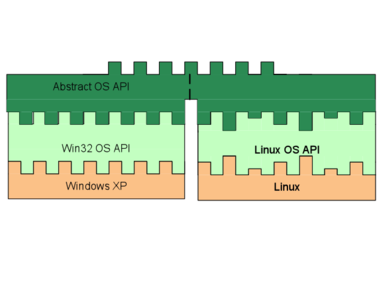
\includegraphics[width=0.6\linewidth]{figs/spm4/osapiModel}
	\caption{Illustration af  OS abstraktion}
	\label{fig:ApiModel}
\end{figure}

\subsubsection{Hvorfor et objekt-orienteret design?}
\begin{itemize}
	\item Lettere af arbejde med, når man er vant til objekter.
	\item Renere kode.
	\begin{itemize}
		\item Koden er mere letlæselig.
		\item Bedre mulighed for at tilføje/ændre i koden.
		\item Bedre \textit{testability}.
		\item Nemt at lave interaktive designs (Eventbaseret programmering).
	\end{itemize}
\end{itemize}

\subsection{Elaborate on the challenge of building it and its currenct design}

\subsubsection{The PIMPL / Cheshire Cat idiom - The how and why}

PIMPL - Pointer to Implementation er et SW programmerings idiom, der fremmer \textit{implementerings abstraktion} for klasser. Lidt på samme måde som interfaces i C\#. Dette gøres vha. en ekstra pointer og funktionskald.

Et eksempel med en \textit{Book} klasse:

\begin{lstlisting}[caption=Klassen Book uden PIMPL, label=code:noPIMP]
class Book
{
public:
	void print();
private:
	std::string  m_Contents;
	std::string  m_Title;
}
\end{lstlisting}

Som det kan ses i kodeudsnit \ref{code:noPIMP}, skal alle Books klienter recompilere hver gang der tilføjes eller ændres i klassen book.

Vi tilføjer et private medlem, \textbf{\textit{class BookImpl}} samt \textbf{\textit{BookImpl* m\_p}}. Vi har også brug for både destructor og constructor nu, for hhv at slette og sætte m\_p! Med PIMPL implementeret får vi da:

\begin{lstlisting}[caption=Klassen Book med PIMPL implementeret, label=code:PIMP]
/* public.h */
class Book
{
public:
	Book();
	~Book();
	void print();
private:
	class BookImpl;
	BookImpl* m_p;
}
\end{lstlisting}

Flere klienter kan nu have deres egen implementering af klassen book. En \textit{privat} implementering kan se således ud:

\begin{lstlisting}[caption=Privat implementering af klassen Book, label=code:PIMP]
Book::Book()
{
	m_p = new BookImpl();
}

Book::~Book()
{
	delete m_p;
}

void Book::print()
{
	m_p->print();
}

/* then BookImpl functions */

void Book::BookImpl::print()
{
	std::cout << "print from BookImpl" << std::endl;
}
\end{lstlisting}

Når vi i vores main ønsker en instans af Book, invokeres det således:
\begin{lstlisting}[caption=Brug af Book klassen i main(), label=code:mainPimpl]
int main()
{
	Book *b = new Book();
	b->print();
	delete b;
}
\end{lstlisting}


\subsubsection{CPU / OS Architecture}

OS Api'er fungerer som et strategy pattern, hvor der vælges strategi alt efter hvilken platform man er på.

\subsection{Effect on design/implementation}

\subsubsection{MQs (Message queues) used with pthreads contra MQ used in OO OS Api}

\subsubsection{RAII in use}
Et idiom brugt til sikker brug af ressourcer, for at undgå memory-leaks. Ideen er at ressourcen allokeres under objektets oprettelse og deallokeres ved destruktion.\\

Kendt under flere navne: 
\begin{itemize}
	\item Resource Acquisition Is Initialization (RAII).
	\item Constructor Acquires, Destructor Releases (CADRe).
	\item Scope-based Resource Management (SBRM).
\end{itemize}



\subsubsection{Using Threads before and now}
Før når vi skulle anvende tråde ville vi gøre noget i stil med det vist i kode udsnit~\ref{code:threads_before}, hvor en tråd erklæres, startes og blokere til den er færdig.

\begin{lstlisting}[caption=Anvendelse af tråde før OSAPI, label=code:threads_before]
pthread_t thread;
pthread_create(&thread, NULL, func, (void*)&arg);
pthread_join(thread, NULL);
\end{lstlisting}

Med OSAPI er det hele mere Objekt Orienteret og generelt nemmere at bruge. Først skal en trådklasse laves (se kode udsnit~\ref{code:threadfunctor}) ved at arve fra \textit{ThreadFunctor} som skulle færdiggøres i øvelse 6.

\begin{lstlisting}[caption=Trådklasse via nedarvning fra ThreadFunctor, label=code:threadfunctor]
#include <osapi/Thread.hpp>

class ThreadClass : public ThreadFunctor 
{
public:
	virtual void run() 
	{
		// job of thread while running
	}
private:
	// class members
};
\end{lstlisting}

Kode udsnit~\ref{code:threads_after} viser hvordan vi nu kan bruge tråde ved hjælp af trådklassen i udsnit~\ref{code:threadfunctor} til let at starte en tråd.

\begin{lstlisting}[caption=Anvendelse af tråde efter OSAPI,
label=code:threads_after,
morekeywords={ThreadClass, Thread, join, start}]
ThreadClass threadclass();	// class to be run in thread
Thread thread(&threadclass);	// thread which the class will run in

thread.start();
thread.join();
\end{lstlisting}

\subsection{UML Diagrams to implementation (class and sequence) - How}

